
\documentclass{article} % For LaTeX2e
\usepackage{iclr2021_conference,times}
\usepackage{graphicx,amsmath,amsthm}

% Optional math commands from https://github.com/goodfeli/dlbook_notation.
%%%% NEW MATH DEFINITIONS %%%%%

\usepackage{amsmath,amsfonts,bm}

% Mark sections of captions for referring to divisions of figures
\newcommand{\figleft}{{\em (Left)}}
\newcommand{\figcenter}{{\em (Center)}}
\newcommand{\figright}{{\em (Right)}}
\newcommand{\figtop}{{\em (Top)}}
\newcommand{\figbottom}{{\em (Bottom)}}
\newcommand{\captiona}{{\em (a)}}
\newcommand{\captionb}{{\em (b)}}
\newcommand{\captionc}{{\em (c)}}
\newcommand{\captiond}{{\em (d)}}

% Highlight a newly defined term
\newcommand{\newterm}[1]{{\bf #1}}


% Figure reference, lower-case.
\def\figref#1{figure~\ref{#1}}
% Figure reference, capital. For start of sentence
\def\Figref#1{Figure~\ref{#1}}
\def\twofigref#1#2{figures \ref{#1} and \ref{#2}}
\def\quadfigref#1#2#3#4{figures \ref{#1}, \ref{#2}, \ref{#3} and \ref{#4}}
% Section reference, lower-case.
\def\secref#1{section~\ref{#1}}
% Section reference, capital.
\def\Secref#1{Section~\ref{#1}}
% Reference to two sections.
\def\twosecrefs#1#2{sections \ref{#1} and \ref{#2}}
% Reference to three sections.
\def\secrefs#1#2#3{sections \ref{#1}, \ref{#2} and \ref{#3}}
% Reference to an equation, lower-case.
\def\eqref#1{equation~\ref{#1}}
% Reference to an equation, upper case
\def\Eqref#1{Equation~\ref{#1}}
% A raw reference to an equation---avoid using if possible
\def\plaineqref#1{\ref{#1}}
% Reference to a chapter, lower-case.
\def\chapref#1{chapter~\ref{#1}}
% Reference to an equation, upper case.
\def\Chapref#1{Chapter~\ref{#1}}
% Reference to a range of chapters
\def\rangechapref#1#2{chapters\ref{#1}--\ref{#2}}
% Reference to an algorithm, lower-case.
\def\algref#1{algorithm~\ref{#1}}
% Reference to an algorithm, upper case.
\def\Algref#1{Algorithm~\ref{#1}}
\def\twoalgref#1#2{algorithms \ref{#1} and \ref{#2}}
\def\Twoalgref#1#2{Algorithms \ref{#1} and \ref{#2}}
% Reference to a part, lower case
\def\partref#1{part~\ref{#1}}
% Reference to a part, upper case
\def\Partref#1{Part~\ref{#1}}
\def\twopartref#1#2{parts \ref{#1} and \ref{#2}}

\def\ceil#1{\lceil #1 \rceil}
\def\floor#1{\lfloor #1 \rfloor}
\def\1{\bm{1}}
\newcommand{\train}{\mathcal{D}}
\newcommand{\valid}{\mathcal{D_{\mathrm{valid}}}}
\newcommand{\test}{\mathcal{D_{\mathrm{test}}}}

\def\eps{{\epsilon}}


% Random variables
\def\reta{{\textnormal{$\eta$}}}
\def\ra{{\textnormal{a}}}
\def\rb{{\textnormal{b}}}
\def\rc{{\textnormal{c}}}
\def\rd{{\textnormal{d}}}
\def\re{{\textnormal{e}}}
\def\rf{{\textnormal{f}}}
\def\rg{{\textnormal{g}}}
\def\rh{{\textnormal{h}}}
\def\ri{{\textnormal{i}}}
\def\rj{{\textnormal{j}}}
\def\rk{{\textnormal{k}}}
\def\rl{{\textnormal{l}}}
% rm is already a command, just don't name any random variables m
\def\rn{{\textnormal{n}}}
\def\ro{{\textnormal{o}}}
\def\rp{{\textnormal{p}}}
\def\rq{{\textnormal{q}}}
\def\rr{{\textnormal{r}}}
\def\rs{{\textnormal{s}}}
\def\rt{{\textnormal{t}}}
\def\ru{{\textnormal{u}}}
\def\rv{{\textnormal{v}}}
\def\rw{{\textnormal{w}}}
\def\rx{{\textnormal{x}}}
\def\ry{{\textnormal{y}}}
\def\rz{{\textnormal{z}}}

% Random vectors
\def\rvepsilon{{\mathbf{\epsilon}}}
\def\rvtheta{{\mathbf{\theta}}}
\def\rva{{\mathbf{a}}}
\def\rvb{{\mathbf{b}}}
\def\rvc{{\mathbf{c}}}
\def\rvd{{\mathbf{d}}}
\def\rve{{\mathbf{e}}}
\def\rvf{{\mathbf{f}}}
\def\rvg{{\mathbf{g}}}
\def\rvh{{\mathbf{h}}}
\def\rvu{{\mathbf{i}}}
\def\rvj{{\mathbf{j}}}
\def\rvk{{\mathbf{k}}}
\def\rvl{{\mathbf{l}}}
\def\rvm{{\mathbf{m}}}
\def\rvn{{\mathbf{n}}}
\def\rvo{{\mathbf{o}}}
\def\rvp{{\mathbf{p}}}
\def\rvq{{\mathbf{q}}}
\def\rvr{{\mathbf{r}}}
\def\rvs{{\mathbf{s}}}
\def\rvt{{\mathbf{t}}}
\def\rvu{{\mathbf{u}}}
\def\rvv{{\mathbf{v}}}
\def\rvw{{\mathbf{w}}}
\def\rvx{{\mathbf{x}}}
\def\rvy{{\mathbf{y}}}
\def\rvz{{\mathbf{z}}}

% Elements of random vectors
\def\erva{{\textnormal{a}}}
\def\ervb{{\textnormal{b}}}
\def\ervc{{\textnormal{c}}}
\def\ervd{{\textnormal{d}}}
\def\erve{{\textnormal{e}}}
\def\ervf{{\textnormal{f}}}
\def\ervg{{\textnormal{g}}}
\def\ervh{{\textnormal{h}}}
\def\ervi{{\textnormal{i}}}
\def\ervj{{\textnormal{j}}}
\def\ervk{{\textnormal{k}}}
\def\ervl{{\textnormal{l}}}
\def\ervm{{\textnormal{m}}}
\def\ervn{{\textnormal{n}}}
\def\ervo{{\textnormal{o}}}
\def\ervp{{\textnormal{p}}}
\def\ervq{{\textnormal{q}}}
\def\ervr{{\textnormal{r}}}
\def\ervs{{\textnormal{s}}}
\def\ervt{{\textnormal{t}}}
\def\ervu{{\textnormal{u}}}
\def\ervv{{\textnormal{v}}}
\def\ervw{{\textnormal{w}}}
\def\ervx{{\textnormal{x}}}
\def\ervy{{\textnormal{y}}}
\def\ervz{{\textnormal{z}}}

% Random matrices
\def\rmA{{\mathbf{A}}}
\def\rmB{{\mathbf{B}}}
\def\rmC{{\mathbf{C}}}
\def\rmD{{\mathbf{D}}}
\def\rmE{{\mathbf{E}}}
\def\rmF{{\mathbf{F}}}
\def\rmG{{\mathbf{G}}}
\def\rmH{{\mathbf{H}}}
\def\rmI{{\mathbf{I}}}
\def\rmJ{{\mathbf{J}}}
\def\rmK{{\mathbf{K}}}
\def\rmL{{\mathbf{L}}}
\def\rmM{{\mathbf{M}}}
\def\rmN{{\mathbf{N}}}
\def\rmO{{\mathbf{O}}}
\def\rmP{{\mathbf{P}}}
\def\rmQ{{\mathbf{Q}}}
\def\rmR{{\mathbf{R}}}
\def\rmS{{\mathbf{S}}}
\def\rmT{{\mathbf{T}}}
\def\rmU{{\mathbf{U}}}
\def\rmV{{\mathbf{V}}}
\def\rmW{{\mathbf{W}}}
\def\rmX{{\mathbf{X}}}
\def\rmY{{\mathbf{Y}}}
\def\rmZ{{\mathbf{Z}}}

% Elements of random matrices
\def\ermA{{\textnormal{A}}}
\def\ermB{{\textnormal{B}}}
\def\ermC{{\textnormal{C}}}
\def\ermD{{\textnormal{D}}}
\def\ermE{{\textnormal{E}}}
\def\ermF{{\textnormal{F}}}
\def\ermG{{\textnormal{G}}}
\def\ermH{{\textnormal{H}}}
\def\ermI{{\textnormal{I}}}
\def\ermJ{{\textnormal{J}}}
\def\ermK{{\textnormal{K}}}
\def\ermL{{\textnormal{L}}}
\def\ermM{{\textnormal{M}}}
\def\ermN{{\textnormal{N}}}
\def\ermO{{\textnormal{O}}}
\def\ermP{{\textnormal{P}}}
\def\ermQ{{\textnormal{Q}}}
\def\ermR{{\textnormal{R}}}
\def\ermS{{\textnormal{S}}}
\def\ermT{{\textnormal{T}}}
\def\ermU{{\textnormal{U}}}
\def\ermV{{\textnormal{V}}}
\def\ermW{{\textnormal{W}}}
\def\ermX{{\textnormal{X}}}
\def\ermY{{\textnormal{Y}}}
\def\ermZ{{\textnormal{Z}}}

% Vectors
\def\vzero{{\bm{0}}}
\def\vone{{\bm{1}}}
\def\vmu{{\bm{\mu}}}
\def\vtheta{{\bm{\theta}}}
\def\va{{\bm{a}}}
\def\vb{{\bm{b}}}
\def\vc{{\bm{c}}}
\def\vd{{\bm{d}}}
\def\ve{{\bm{e}}}
\def\vf{{\bm{f}}}
\def\vg{{\bm{g}}}
\def\vh{{\bm{h}}}
\def\vi{{\bm{i}}}
\def\vj{{\bm{j}}}
\def\vk{{\bm{k}}}
\def\vl{{\bm{l}}}
\def\vm{{\bm{m}}}
\def\vn{{\bm{n}}}
\def\vo{{\bm{o}}}
\def\vp{{\bm{p}}}
\def\vq{{\bm{q}}}
\def\vr{{\bm{r}}}
\def\vs{{\bm{s}}}
\def\vt{{\bm{t}}}
\def\vu{{\bm{u}}}
\def\vv{{\bm{v}}}
\def\vw{{\bm{w}}}
\def\vx{{\bm{x}}}
\def\vy{{\bm{y}}}
\def\vz{{\bm{z}}}

% Elements of vectors
\def\evalpha{{\alpha}}
\def\evbeta{{\beta}}
\def\evepsilon{{\epsilon}}
\def\evlambda{{\lambda}}
\def\evomega{{\omega}}
\def\evmu{{\mu}}
\def\evpsi{{\psi}}
\def\evsigma{{\sigma}}
\def\evtheta{{\theta}}
\def\eva{{a}}
\def\evb{{b}}
\def\evc{{c}}
\def\evd{{d}}
\def\eve{{e}}
\def\evf{{f}}
\def\evg{{g}}
\def\evh{{h}}
\def\evi{{i}}
\def\evj{{j}}
\def\evk{{k}}
\def\evl{{l}}
\def\evm{{m}}
\def\evn{{n}}
\def\evo{{o}}
\def\evp{{p}}
\def\evq{{q}}
\def\evr{{r}}
\def\evs{{s}}
\def\evt{{t}}
\def\evu{{u}}
\def\evv{{v}}
\def\evw{{w}}
\def\evx{{x}}
\def\evy{{y}}
\def\evz{{z}}

% Matrix
\def\mA{{\bm{A}}}
\def\mB{{\bm{B}}}
\def\mC{{\bm{C}}}
\def\mD{{\bm{D}}}
\def\mE{{\bm{E}}}
\def\mF{{\bm{F}}}
\def\mG{{\bm{G}}}
\def\mH{{\bm{H}}}
\def\mI{{\bm{I}}}
\def\mJ{{\bm{J}}}
\def\mK{{\bm{K}}}
\def\mL{{\bm{L}}}
\def\mM{{\bm{M}}}
\def\mN{{\bm{N}}}
\def\mO{{\bm{O}}}
\def\mP{{\bm{P}}}
\def\mQ{{\bm{Q}}}
\def\mR{{\bm{R}}}
\def\mS{{\bm{S}}}
\def\mT{{\bm{T}}}
\def\mU{{\bm{U}}}
\def\mV{{\bm{V}}}
\def\mW{{\bm{W}}}
\def\mX{{\bm{X}}}
\def\mY{{\bm{Y}}}
\def\mZ{{\bm{Z}}}
\def\mBeta{{\bm{\beta}}}
\def\mPhi{{\bm{\Phi}}}
\def\mLambda{{\bm{\Lambda}}}
\def\mSigma{{\bm{\Sigma}}}

% Tensor
\DeclareMathAlphabet{\mathsfit}{\encodingdefault}{\sfdefault}{m}{sl}
\SetMathAlphabet{\mathsfit}{bold}{\encodingdefault}{\sfdefault}{bx}{n}
\newcommand{\tens}[1]{\bm{\mathsfit{#1}}}
\def\tA{{\tens{A}}}
\def\tB{{\tens{B}}}
\def\tC{{\tens{C}}}
\def\tD{{\tens{D}}}
\def\tE{{\tens{E}}}
\def\tF{{\tens{F}}}
\def\tG{{\tens{G}}}
\def\tH{{\tens{H}}}
\def\tI{{\tens{I}}}
\def\tJ{{\tens{J}}}
\def\tK{{\tens{K}}}
\def\tL{{\tens{L}}}
\def\tM{{\tens{M}}}
\def\tN{{\tens{N}}}
\def\tO{{\tens{O}}}
\def\tP{{\tens{P}}}
\def\tQ{{\tens{Q}}}
\def\tR{{\tens{R}}}
\def\tS{{\tens{S}}}
\def\tT{{\tens{T}}}
\def\tU{{\tens{U}}}
\def\tV{{\tens{V}}}
\def\tW{{\tens{W}}}
\def\tX{{\tens{X}}}
\def\tY{{\tens{Y}}}
\def\tZ{{\tens{Z}}}


% Graph
\def\gA{{\mathcal{A}}}
\def\gB{{\mathcal{B}}}
\def\gC{{\mathcal{C}}}
\def\gD{{\mathcal{D}}}
\def\gE{{\mathcal{E}}}
\def\gF{{\mathcal{F}}}
\def\gG{{\mathcal{G}}}
\def\gH{{\mathcal{H}}}
\def\gI{{\mathcal{I}}}
\def\gJ{{\mathcal{J}}}
\def\gK{{\mathcal{K}}}
\def\gL{{\mathcal{L}}}
\def\gM{{\mathcal{M}}}
\def\gN{{\mathcal{N}}}
\def\gO{{\mathcal{O}}}
\def\gP{{\mathcal{P}}}
\def\gQ{{\mathcal{Q}}}
\def\gR{{\mathcal{R}}}
\def\gS{{\mathcal{S}}}
\def\gT{{\mathcal{T}}}
\def\gU{{\mathcal{U}}}
\def\gV{{\mathcal{V}}}
\def\gW{{\mathcal{W}}}
\def\gX{{\mathcal{X}}}
\def\gY{{\mathcal{Y}}}
\def\gZ{{\mathcal{Z}}}

% Sets
\def\sA{{\mathbb{A}}}
\def\sB{{\mathbb{B}}}
\def\sC{{\mathbb{C}}}
\def\sD{{\mathbb{D}}}
% Don't use a set called E, because this would be the same as our symbol
% for expectation.
\def\sF{{\mathbb{F}}}
\def\sG{{\mathbb{G}}}
\def\sH{{\mathbb{H}}}
\def\sI{{\mathbb{I}}}
\def\sJ{{\mathbb{J}}}
\def\sK{{\mathbb{K}}}
\def\sL{{\mathbb{L}}}
\def\sM{{\mathbb{M}}}
\def\sN{{\mathbb{N}}}
\def\sO{{\mathbb{O}}}
\def\sP{{\mathbb{P}}}
\def\sQ{{\mathbb{Q}}}
\def\sR{{\mathbb{R}}}
\def\sS{{\mathbb{S}}}
\def\sT{{\mathbb{T}}}
\def\sU{{\mathbb{U}}}
\def\sV{{\mathbb{V}}}
\def\sW{{\mathbb{W}}}
\def\sX{{\mathbb{X}}}
\def\sY{{\mathbb{Y}}}
\def\sZ{{\mathbb{Z}}}

% Entries of a matrix
\def\emLambda{{\Lambda}}
\def\emA{{A}}
\def\emB{{B}}
\def\emC{{C}}
\def\emD{{D}}
\def\emE{{E}}
\def\emF{{F}}
\def\emG{{G}}
\def\emH{{H}}
\def\emI{{I}}
\def\emJ{{J}}
\def\emK{{K}}
\def\emL{{L}}
\def\emM{{M}}
\def\emN{{N}}
\def\emO{{O}}
\def\emP{{P}}
\def\emQ{{Q}}
\def\emR{{R}}
\def\emS{{S}}
\def\emT{{T}}
\def\emU{{U}}
\def\emV{{V}}
\def\emW{{W}}
\def\emX{{X}}
\def\emY{{Y}}
\def\emZ{{Z}}
\def\emSigma{{\Sigma}}

% entries of a tensor
% Same font as tensor, without \bm wrapper
\newcommand{\etens}[1]{\mathsfit{#1}}
\def\etLambda{{\etens{\Lambda}}}
\def\etA{{\etens{A}}}
\def\etB{{\etens{B}}}
\def\etC{{\etens{C}}}
\def\etD{{\etens{D}}}
\def\etE{{\etens{E}}}
\def\etF{{\etens{F}}}
\def\etG{{\etens{G}}}
\def\etH{{\etens{H}}}
\def\etI{{\etens{I}}}
\def\etJ{{\etens{J}}}
\def\etK{{\etens{K}}}
\def\etL{{\etens{L}}}
\def\etM{{\etens{M}}}
\def\etN{{\etens{N}}}
\def\etO{{\etens{O}}}
\def\etP{{\etens{P}}}
\def\etQ{{\etens{Q}}}
\def\etR{{\etens{R}}}
\def\etS{{\etens{S}}}
\def\etT{{\etens{T}}}
\def\etU{{\etens{U}}}
\def\etV{{\etens{V}}}
\def\etW{{\etens{W}}}
\def\etX{{\etens{X}}}
\def\etY{{\etens{Y}}}
\def\etZ{{\etens{Z}}}

% The true underlying data generating distribution
\newcommand{\pdata}{p_{\rm{data}}}
% The empirical distribution defined by the training set
\newcommand{\ptrain}{\hat{p}_{\rm{data}}}
\newcommand{\Ptrain}{\hat{P}_{\rm{data}}}
% The model distribution
\newcommand{\pmodel}{p_{\rm{model}}}
\newcommand{\Pmodel}{P_{\rm{model}}}
\newcommand{\ptildemodel}{\tilde{p}_{\rm{model}}}
% Stochastic autoencoder distributions
\newcommand{\pencode}{p_{\rm{encoder}}}
\newcommand{\pdecode}{p_{\rm{decoder}}}
\newcommand{\precons}{p_{\rm{reconstruct}}}

\newcommand{\laplace}{\mathrm{Laplace}} % Laplace distribution

\newcommand{\E}{\mathbb{E}}
\newcommand{\Ls}{\mathcal{L}}
\newcommand{\R}{\mathbb{R}}
\newcommand{\emp}{\tilde{p}}
\newcommand{\lr}{\alpha}
\newcommand{\reg}{\lambda}
\newcommand{\rect}{\mathrm{rectifier}}
\newcommand{\softmax}{\mathrm{softmax}}
\newcommand{\sigmoid}{\sigma}
\newcommand{\softplus}{\zeta}
\newcommand{\KL}{D_{\mathrm{KL}}}
\newcommand{\Var}{\mathrm{Var}}
\newcommand{\standarderror}{\mathrm{SE}}
\newcommand{\Cov}{\mathrm{Cov}}
% Wolfram Mathworld says $L^2$ is for function spaces and $\ell^2$ is for vectors
% But then they seem to use $L^2$ for vectors throughout the site, and so does
% wikipedia.
\newcommand{\normlzero}{L^0}
\newcommand{\normlone}{L^1}
\newcommand{\normltwo}{L^2}
\newcommand{\normlp}{L^p}
\newcommand{\normmax}{L^\infty}

\newcommand{\parents}{Pa} % See usage in notation.tex. Chosen to match Daphne's book.

\DeclareMathOperator*{\argmax}{arg\,max}
\DeclareMathOperator*{\argmin}{arg\,min}

\DeclareMathOperator{\sign}{sign}
\DeclareMathOperator{\Tr}{Tr}
\let\ab\allowbreak


\newtheorem{definition}{Definition}


\usepackage{hyperref}
\usepackage{url}


\title{An invitation to singular learning theory}

% Authors must not appear in the submitted version. They should be hidden
% as long as the \iclrfinalcopy macro remains commented out below.
% Non-anonymous submissions will be rejected without review.

\author{Antiquus S.~Hippocampus, Natalia Cerebro \& Amelie P. Amygdale \thanks{ Use footnote for providing further information
about author (webpage, alternative address)---\emph{not} for acknowledging
funding agencies.  Funding acknowledgements go at the end of the paper.} \\
Department of Computer Science\\
Cranberry-Lemon University\\
Pittsburgh, PA 15213, USA \\
\texttt{\{hippo,brain,jen\}@cs.cranberry-lemon.edu} \\
\And
Ji Q. Ren \& Yevgeny LeNet \\
Department of Computational Neuroscience \\
University of the Witwatersrand \\
Joburg, South Africa \\
\texttt{\{robot,net\}@wits.ac.za} \\
\AND
Coauthor \\
Affiliation \\
Address \\
\texttt{email}
}

\RequirePackage{algorithm}
\RequirePackage{algorithmic}

% The \author macro works with any number of authors. There are two commands
% used to separate the names and addresses of multiple authors: \And and \AND.
%
% Using \And between authors leaves it to \LaTeX{} to determine where to break
% the lines. Using \AND forces a linebreak at that point. So, if \LaTeX{}
% puts 3 of 4 authors names on the first line, and the last on the second
% line, try using \AND instead of \And before the third author name.

\def\be{\begin{equation}}
\def\ee{\end{equation}}
\newcommand{\fix}{\marginpar{FIX}}
\newcommand{\new}{\marginpar{NEW}}
\def\l{\,|\,}
\def\lto{\longrightarrow}

\newtheorem{theorem}{Theorem}[section]
\newtheorem{lemma}[theorem]{Lemma}
\newtheorem{remark}[theorem]{Remark}
\newtheorem{example}[theorem]{Example}

%\iclrfinalcopy % Uncomment for camera-ready version, but NOT for submission.
\begin{document}


\maketitle

\begin{abstract}
The abstract paragraph should be indented 1/2~inch (3~picas) on both left and
right-hand margins. Use 10~point type, with a vertical spacing of 11~points.
The word \textsc{Abstract} must be centered, in small caps, and in point size 12. Two
line spaces precede the abstract. The abstract must be limited to one
paragraph.
\end{abstract}

\section{Introduction}

It has been understood for close to twenty years that neural networks are singular statistical models \cite{amari_learning_2003, watanabe_almost_2007}.
The study of singular models, also known as singular learning theory \citep{watanabe_algebraic_2009}, requires very different tools from the study of regular models. The breadth of knowledge demanded by singular learning theory -- Bayesian statistics, empirical processes, algebraic geometry, and mathematical physics -- is rewarded with profound and surprising results which reveal singular models are different from regular models in practically important ways.


Despite its potential for addressing fundamental mysteries in deep learning, singular learning theory appears to have made little inroads into the developing canon of deep learning theory. In this note we present an invitation to key ideas of singular learning theory via a mix of theory and simple experiments, in the hope of making the topic accessible to a wider audience. 
%We also point out some misconceptions in the literature, on which light is shed by the theory.
%We use $p$ to stand for a class of statistical models, determined by neural networks parametrised by weights $w \in W$, $q$ to stand for the true distribution (from which a finite training set is sampled) and $\varphi$ to stand for a prior over the weights.
Each section of the paper illustrates one key take-away idea:

\begin{itemize}
    \item \textbf{Neural networks are singular models} (Section \ref{section:nn_singular}). A many-layered neural network statistical model is non-identifiable and has degenerate Fisher information matrix \emph{at every point of the parameter space}. Classical tools from statistical inference are hence inappropriate for neural networks, e.g., one should not ``divide" by the determinant of the Hessian in deep learning. 
    \item \textbf{The real log canonical threshold (RLCT) is the correct way to count the effective number of parameters in a deep neural network.} (Section \ref{section:no_flat_minima}). 
    To every (model, truth, prior) triplet is associated a birational invariant known as the real log canonical threshold (RLCT). The RLCT can be understood as the number of normal directions to the set of true parameters. We will explain why this matters much more than the curvature of those directions (as measured for example by eigenvalues of the Hessian), laying bare some of the confusion over ``flat'' minima in deep learning 
    \item \textbf{For singular models, Bayes predictive distribution is superior to MAP and MLE} (Section \ref{section:gen_error}). In regular statistical models, MAP, MLE, and the Bayes predictive distribution share the same leading term in the asymptotic expansion of the Kullback-Leibler generalizatoin error. This is not so in singular models. We illustrate in our experiments that even ``being Bayesian'' in just the final layers improves generalisation over MAP. Our experiments further confirm that the Laplace approximations of the predictive distribution is indeed not appropriate in deep learning.
    \item \textbf{The complexity of a singularity is inversely proportional to the RLCT} (Section \ref{section:simple_func}). In singular models the RLCT depends on the (model, truth, prior) triple whereas in regular models it depends only on the (model, prior) pair.
     %under a hypothesis of realisability. 
     We verify this experimentally with a simple family of ReLU networks. Furthermore we empirically observe that the complexity of a singularity is inversely proportional to the RLCT.
\end{itemize}

\section{Singular Learning Theory}

In classical learning theory, generalisation is explained by measures of capacity such as the $l_2$ norm, Radamacher complexity, and VC dimension \citep{bousquet2003introduction}. It has become clear however that these measures are unable to account for the empirical success of deep neural networks \citep{zhang_understanding_2017}. Rethinking generalisation will likely require devising capacity measures suitable to the peculiarities of deep learning, e.g. non-identifiability and degenerate Fisher information matrix. 

To understand why classical measures of capacity fail to say anything meaningful about deep neural networks (DNN), it is important to distinguish between two different types of statistical models. Suppose we are interested in estimating the true (unknown) conditional distribution $q(y|x)$ with a class of models $\{p(y|x,w): w \in W\}$ where $W \subset \mathbb R^d$ is the parameter space. Let 
$$
W_0 = \{w \in W: p(y|x,w)=q(y|x)\}
$$
 be the set of true parameters. 
Following the conventions in \cite{watanabe_algebraic_2009}, we have the following bifurcation of statistical models:
\begin{definition}
A statistical model $p(y|x,w)$ is called \textbf{regular} if it is 1) identifiable, i.e, if $W_0$ is a singleton, and 2) has positive-definite Fisher information matrix. A statistical model is called \textbf{strictly singular} if it is not regular. 
%{\cite[Theorem 7.2]{watanabe_algebraic_2009}}.
\end{definition}

% \begin{definition}[Singular model]
% A singular statistical model is either a regular model or a strictly singular model. 
% \end{definition}

Let  $\varphi(w)$ be a prior on the model parameters $w$.
To every model-truth-prior triplet, we can associate the zeta function
\begin{equation}
\zeta(z) = \int K(w)^z \varphi(w) \,dw, \quad z \in \mathbb C,
\end{equation} 
where $K(w)$ is the Kullback-Leibler divergence between the model $p(y|x,w)$ and the true distribution $q(y|x)$:
\begin{equation}
    K(w) := \int \!\int q(y|x) \log \frac{ q(y|x) }{ p(y|x,w) } q(x) \,dx \,dy.
\end{equation}
Then to every triplet of model-truth-prior, we can associate the following central quantity of singular learning theory:

\begin{definition}[Real log canonical threshold (RLCT)]
For a model-truth-prior triplet $(p(y|x,w),q(y|x),\varphi)$, let $-\lambda$ be the maximum pole of the corresponding zeta function. We call $\lambda$ the real log canonical threshold of the model-truth-prior triplet.
\label{def:RLCT}
\end{definition}

By {\citet[Theorem 6.4]{watanabe_algebraic_2009}}, the RLCT is equal to $d/2$ in regular statistical models. Furthermore the RLCT is bounded above by $d/2$ in strictly singular models, if \textit{realizability} holds:
 \begin{definition}
	We say $q(y|x)$ is \textbf{realizable} by the model class $\{p(y|x,w)\}$ if $W_0$ is non-empty.
\end{definition}
The condition of realizability will be critical to the standard results in singular learning theory. Modifications to the theory are needed in the case that $q(y|x)$ is not realisable, see the more general condition called relatively finite variance in \citet{watanabe_mathematical_2018}.

% The work of Sumio Watanabe on singular learning theory \cite{watanabe_algebraic_2009} suggests that the \textit{real log canonical threshold} (RLCT) of a deep neural network is suitable for measuring its effective number of parameters (see Section ???). 
\paragraph{RLCT as a measure of model complexity}
One of the most accessible results in singular learning theory is the work related to the widely-applicable Bayesian information criterion (WBIC) \citet{watanabe_widely_2013}. We explain briefly the developments here since many in the deep learning community may not be aware of this work.

Let $\mathcal D_n =  \{(x_i,y_i)\}_{i=1}^n$ be a dataset of input-output pairs.  
Let $L_n(w)$ be the negative log likelihood
\begin{equation}
L_n(w) = -\frac{1}{n} \sum_{i=1}^n \log p(y_i |x_i, w)
\label{eq:nll}
\end{equation}
The marginal likelihood of a model $\{p(y|x,w): w \in W\}$ is given by
$$
p(\mathcal D_n) = \int_W p(\mathcal D_n|w) \varphi(w) \,dw.
$$
Since the marginal likelihood is an intractable integral over the parameter space of the model, one needs to consider some approximation.

Recall that the well-known Bayesian Information Criterion (BIC) derives from an asymptotic approximation of the negative log marginal likelihood, $-\log p(\mathcal D_n)$, using the Laplace approximation, leading to
\[
\operatorname{BIC} = nL_n( w_{mle}) + \frac{d}{2} \log n.
\]
Since we want the marginal likelihood of the data for some given model to be \textit{high}, we want the negative log marginal likelihood to be \textit{low}. Thus when $d$ is extremely large as is the case in deep neural networks, one should almost never adopt a deep network according to the BIC. 
%(aka the log marginal likelihood, aka the free energy). 
% Given two statistical models of a data source, one should choose (all else being equal) the one with higher model evidence. 

However, this argument contains a serious mathematical error: the Laplace approximation used to derive BIC only applies to \emph{regular} statistical models, and deep neural networks are not regular. Deep neural networks are \textit{strictly singular} as we illustrated in Section \ref{section:nn_singular}. 
If we have realizability (along with a few more technical conditions), the correct criterion for both regular and strictly singular models was shown in \citet{watanabe_widely_2013} to be 
\begin{equation}
nL_n(w_0) + \lambda \log n,
\label{logmarginal_rlct}
\end{equation}
where $w_0 \in W_0$ and $\lambda$ is the RLCT. 
The RLCT is a birational invariant \citep{kollar_birational_1998} that directly measures the complexity of singularities in the model. Since more complex singularities lead to smaller values of $\lambda$, which we illustrate in Section \ref{section:simple_func}, and deep learning models are highly singular, it is possible for deep neural networks to have high marginal likelihood -- consistent with their empirical success. 


??? needs a better transition ???
Capacity measures for explaining the generalization of deep neural networks is an active area of research \cite{neyshabur_exploring_2017}. It is still common practice to work with degenerate Hessians in proposing capacity measures \cite{thomas_information_2019}. Another common mistake is to perform the Laplace approximation for singular neural networks. For instance, \citet{zhang_energyentropy_2018} posit a relationship between the generalisation error of the full Bayes predictor and an entropy term (Eq (14)). Le and Smith \cite{le_bayesian_2018} do something very similar. These works rely on Laplace approximation (saddlepoint approximation) of the intractable posterior distribution. ???Also discuss the following works \cite{maddox_rethinking_2020}, \cite{gao_degrees_2016}, \cite{sun_lightlike_2020}.???


\subsection{Neural networks are strictly singular}
\label{section:nn_singular}

A ReLU network of depth $k$ is a function $f: \mathbb{R}^N \lto \mathbb{R}^M$ of the form
\[
f = A_k \circ \operatorname{ReLU}_{k-1} \circ A_{k-1} \cdots \operatorname{ReLU}_1 \circ A_1
\]
where the $A_i: \mathbb{R}^{d_i} \lto \mathbb{R}^{d_{i+1}}$ are affine functions and the function $\operatorname{ReLU}_i: \mathbb{R}^{d_{i+1}} \lto \mathbb{R}^{d_{i+1}}$ is coordinate-wise $\operatorname{ReLU}$. Let $W$ be a compact subspace of the space $\mathbb{R}^D$ containing the origin, where $\mathbb{R}^D$ is the space of sequences affine functions $(A_i)_{i=1}^k$ with coordinates denoted $w_1,\ldots,w_D$, so that $f$ may be viewed as a function $f: \mathbb{R}^N \times W \lto \mathbb{R}^M$. We define
\[
p(y|x,w) = \frac{1}{(2 \pi)^{M/2}} \exp\Big(-\tfrac{1}{2} \| y - f(x,w) \|^2 \Big)\,.
\]
The Fisher information matrix is the matrix valued function on $W$ defined by
\[
I(w)_{ij} = \int\!\int \frac{\partial}{\partial w_i}[ \log p(y|x,w) ] \frac{\partial}{\partial w_j}[ \log p(y|x,w) ] p(y|x,w) q(x) dx dy
\]
if this integral is finite. Then it is a standard calculation that
\begin{equation}\label{eq:fisher_relu}
I(w)_{ij} = \frac{1}{2^{(M-3)/2} \pi^{(M-2)/2}} \int_{\mathbb{R}^N} \Big\langle \frac{\partial}{\partial w_i} f(x,w), \frac{\partial}{\partial w_j} f(x,w) \Big\rangle q(x) dx
\end{equation}
where $\langle -, - \rangle$ denotes the dot product on $\mathbb{R}^M$. Given $w \in W$ we let $\mathcal{D}(w)$ denote the complement in $\mathbb{R}^N$ of the union over all hidden nodes of the decision boundary at that node (clarify). Since each of these decision boundaries is a hyperplane, $\mathcal{D}(w)$ is a disjoint union of finitely many open chambers. The partial derivative with respect to $\frac{\partial}{\partial w_j}$ of $f: \mathbb{R}^N \times W \lto \mathbb{R}^M$ exists at any point $(x,w)$ with $x \in \mathcal{D}(w)$ and \eqref{eq:fisher_relu} is to be interpreted as a sum over integrals over chambers.

\begin{lemma}\label{lemma:reln} For any hidden node in the network with coordinates $(a_k)_k$ for the incoming weights, $(b_i)_i$ for the outgoing weights and $c$ for the bias
\begin{align*}
\Big\{ \sum_k a_{k}\frac{\partial}{\partial a_k} + c \frac{\partial}{\partial c}-\sum_{i} b_i\frac{\partial}{\partial b_i} \Big\} f = 0.
\end{align*}
\end{lemma}
\begin{proof}
Let $e_i$ denote unit vectors and $H(x)=\frac{d}{dx}\operatorname{ReLU}(x)$. Let $u$ and $a$ denote the value of node before and after activation, respectively $u =\sum_k w_k a_{k}^{l-1}+b_{j}^{l}$ and $a_{j}^{l} =\operatorname{ReLU}(u_{j}^{l})$. Then
\begin{align*}
\frac{\partial f}{\partial q_i}&=\frac{\partial y}{\partial u}u_{j}^{l}H(u_{j}^{l})e_{i}\\
\frac{\partial y}{\partial w_{jk}^{l}}&=\frac{\partial y}{\partial u^{l+1}}\frac{\partial u^{l+1}}{\partial w_{jk}^{l}}=\frac{\partial y}{\partial u^{l+1}}\sum_{i=1}^{d_{l+1}}w_{ij}^{l+1}a_{k}^{l-1}H(u_{j}^{l})e_{i}.\\
\frac{\partial y}{\partial b_{j}^{l}}&=\frac{\partial y}{\partial u^{l+1}}\frac{\partial u^{l+1}}{\partial b_{j}^{l}}=\frac{\partial y}{\partial u^{l+1}}\sum_{i=1}^{d_{l+1}}w_{ij}^{l+1}H(u_{j}^{l})e_{i}.
\end{align*}
The claim immediately follows (TODO: fix notation).
\end{proof}

\begin{lemma} The matrix $I(w)$ is degenerate at every nonzero point of $W$.
\end{lemma}
\begin{proof}
Let $w \in W$ be given, and choose a hidden node where at least one of the incident weights (or bias) is nonzero. Then Lemma \ref{lemma:reln} gives a nontrivial linear dependence relation $\sum_i \lambda_i \frac{\partial}{\partial w_i} f = 0$ as functions on $\mathbb{R}^N$. The rows of $I(w)$ satisfy the same linear dependence relation.
\end{proof}

The well-known positive scale invariance of ReLU networks is responsible for the linear dependence of Lemma \ref{lemma:reln}, but this is only one source of degeneracy or singularity in ReLU networks. As we show in Section \ref{??} even once this symmetry is ``fixed'' there is additional degeneracy (as measured by the RLCT).

\begin{remark} (cleanup)
e.g. Amari, this lightlike-neuromanifold thing) that make this minimal singularity assumption are just irrelevant to deep learning.
\end{remark}

\newpage

\section{Volume dimension, effective degrees of freedom, and flatness}
\label{section:no_flat_minima}

The easiest way to understand the RLCT is as a volume dimension \citep[Theorem 7.1]{watanabe_algebraic_2009}. To explain, we begin with the special case of a singular statistical model with the property that in a neighborhood of every point $w_0 \in W_0$ the Kullback-Liebler distance has an expression in local coordinates
\begin{equation}\label{eq:local_Kw}
K(w) = \sum_{i=1}^{d'} \lambda_i w_i^2
\end{equation}
where the coefficients $\lambda_1,\ldots,\lambda_{d'} > 0$ depend on $w_0$. It follows that the set $W_0 \subseteq W$ of true parameters is a regular submanifold of codimension $d'$ (that is, $W_0$ is a manifold of dimension $d - d'$ where $W$ has dimension $d$). Under this hypothesis there are, near each true parameter $w_0 \in W_0$, exactly $d - d'$ directions in which $w_0$ can be varied without changing the model $p(y|x,w)$ and $d'$ directions in which varying the parameters does change the model. In this sense, there are $d'$ \emph{effective parameters} (or \emph{effective degrees of freedom}) near $w_0$. This effective dimension can be computed by an integral. To see this, define the volume of the set of ``almost true'' parameters near $w_0$ to be
%This is not true in general, and it is not true of deep neural networks, but it is true of regular models with $d' = 0$ (the set of true parameters is a set of isolated points) and for singular models such as reduced rank regression with $d' > 0$.
\begin{equation}\label{eq:true_param}
V(t) = \int_{K(w) < t} \varphi(w) dw\,.
\end{equation}
As long as the prior $\varphi(w)$ is nonzero on $W_0$ it does not affect the relevant features of the volume, so we may assume $\varphi$ is constant on the region of integration in the first $d'$ directions and normal in the remaining directions, so up to a constant depending only on $d'$ we have
\begin{equation}\label{eq:volume_singular}
V(t) \propto \frac{t^{d'/2}}{\sqrt{\lambda_1 \cdots \lambda_{d'}}}
\end{equation}
and we can extract the exponent of $t$ in this volume in the limit
\be\label{eq:limit_volumedim}
d' = 2 \lim_{t \to 0} \frac{\log\big\{V(at)/V(t)\big\}}{\log(a)}
\ee
for any $a > 0$, $a \neq 1$. The right hand side of (\ref{eq:limit_volumedim}) is the \emph{volume dimension} associated to $K$ and $w_0$.

More generally, we can consider a model which in which $K(w)$ has the form (\ref{eq:local_Kw})  near each point of $W_0$ but where the codimension $d'$ (and hence the volume dimension) varies from point to point (for instance $W_0$ might be a disjoint union of two regular submanifolds). What are we to make of such a situation? Since two true parameters with different volume dimensions still determine the same model, the significance of this situation requires explanation.

We take the point of view that in deep learning it is not meaningful to talk about \emph{points} $w \in W$ as this would suggest an inference procedure of infinite precision. The only ``physically'' meaningful quantities are distributions $\psi(w)$ over $W$ and the associated predictive distributions
\[
p^*_\psi(y|x) = \int p(y|x,w) \psi(w) dw\,.
\]
While two parameters $w_0, w_1$ with volume dimensions $d'_0, d'_1$ determine the same model, if the predictive distributions $p^*_{\psi_1}(y|x)$ and $p^*_{\psi_2}(y|x)$ are essentially different for $\psi_i$ arbitrarily concentrated around $w_i$ then the two parameters are, in a deeper sense, not equivalent. For example, suppose the statistical model is of exponential form, as with the models defined in Section \ref{??} associated to two-layer ReLU networks. 

Given a fixed dataset $D_n = \{ (x_i,y_i) \}_{i=1}^n$ sampled from the true distribution we consider the expected squared error over the dataset
\[
E(T) = \mathbb{E}_w^T\Big[ \sum_{i=1}^n \| y_i - f(x_i, w) \|^2 \Big]
\]
where $w$ from the posterior at temperature $T$. This quantity is a random variable, which depends on the dataset $D_n$ the temperature $T$ and the prior $\varphi(w)$ that is placed on the parameters. The temperature controls how finely parameters are distinguished: at high temperature points with high posterior probability are barely distinguishable from points with low probability, and as $T \lto 0$ all the probability concentrates around true parameters. Consider the change $\Delta E = E(T + \Delta T) - E(T)$ resulting from an increase in the temperature. This is a measure of sensitivity of the performance of the predictive distribution to temperature. If our prior $\varphi = \psi_i$ is concentrated near a point $w_i \in W_0$ of volume dimension $d'_i$, then it can be shown that
\[
\Delta E \approx \frac{d'_i}{2} \Delta T
\]
Hence if $d'_0 < d'_1$ then the model we obtain by integrating near $w_0$ will have an error which increases less quickly with temperature. From the point of view of statistical learning two true parameters with different volume dimensions are not equivalent.

\textbf{General theory}. With this in mind the conceptual link between volume dimension and generalisation error can be seen as follows.Singular learning theory bears out a general connection between $\Delta E / \Delta T$, the Bayesian generalisation error and the volume dimension. For any singular model satisfying some natural conditions \citep[Theorem 7.1]{watanabe_algebraic_2009} shows that
\[
V(t) = c t^\lambda (- \log t)^{m-1} + o( t^\lambda ( - \log t)^{m-1})
\]
for a positive rational number $\lambda$, namely the \emph{Real Log Canonical Threshold} (RLCT). It follows that $\lambda$ is the volume dimension computed by (\ref{eq:volume_singular}) and that $\lambda = d'/2$ in the situation considered above. 

\begin{remark}
It is folklore in the deep learning community that flatter minima have better generalisation properties \citep{hinton_keeping_1993, hochreiter1997flat} and this claim has been revisited in recent years \citep{chaudhari2019entropy, smith2017bayesian, jastrzkebski2017three, Zhang:2018MolPh.116.3214Z}. 

The intuition of \citep{hochreiter1997flat} is incorrect. Their measure of entropy is something like
\[
- \log V(E_{tol}) = const + \sum_i \tfrac{1}{2} \log \lambda_i
\]
where the $t^{d'/2}$ should be thought of as the volume of the enclosing ball (i.e. think of cutting out all ``almost true'' parameters within an epsilon ball of some radius around $w_0$). You can get rid of the constant terms by defining your denominator in the volume, so that this calculates the entropy to be a sum of the $\log \lambda_i$. However this doesn't get the correct behaviour of the generalisation error. This corresponds to an error analysis that considers uncorrelated errors $\Delta w_i$ of the same size.

 lower order terms of the asymptotic expansion of the Bayes free energy \citep[\S 3.1]{Balasubramanian:1996cond.mat..1030B}
\end{remark}

% Note that in comparing two regular models with parameter space $W \subseteq \mathbb{R}^d$, both of which have volume dimension $d/2$, the Hessian determinant is relevant to compare how the respective volumes of almost true parameters vary with $t$. But in comparing two minimally singular models with Hessian determinants of rank $d', d''$ the behaviour of the volume depends much more strongly on the dimensions $d'/2, d''/2$ than it does on the eigenvalues.
% From a theoretical point of view the exponent $d/2$ appears as the leading $O(\log n)$ term in the asymptotic expansion of the Bayes free energy and the Hessian determinant appears in the next $O(1)$ term, where $n$ is the size of a dataset . The upshot of this is that if two regular models have parameter spaces of dimension $d_1 < d_2$ one should prefer the model class of dimension $d_1$ (assuming both can perfectly fit the data) but if $d_1 = d_2$ then it may be appropriate to compare models on the basis of their curvature at the true parameter.

% What kind of space is the set of true parameters of a singular statistical model? In modern mathematics we generally think of spaces as a pair consisting of a topological space $X$ and a sheaf of rings, which for every open subset $U \subseteq X$ picks out a certain class of continuous functions $U \lto \mathbb{R}$. In the theory of smooth or analytic manifolds, for instance, these would be the $C^\infty$ or $C^\omega$ functions, while in algebraic geometry these would be the regular functions. Historically statistical learning theory and machine learning has mostly employed concepts of space from differential geometry, where this sheaf can be safely left implicit: if $X \subseteq \mathbb{R}^D$ is a regular submanifold, the manifold structure on $X$ can be recovered from the \emph{set} $X$ and the manifold structure on $\mathbb{R}^D$. However in algebraic geometry a closed subspace does \emph{not} have an unambiguous structure as a space in its own right:

%\begin{example} The zero locus of $x$ and $x^2$ in $\mathbb{R}^2$ have the same underlying set, but as schemes the former is smooth and has coordinate ring $\mathbb{R}[x,y]/x \cong \mathbb{R}[y]$ while the latter is singular and has coordinate ring $\mathbb{R}[x,y]/x^2$. Singularity vs regularity is \emph{not a property of the set} but the function whose zero locus the set is.
%\end{example}

\section{Generalization}\label{section:gen_error}
In the Bayesian paradigm, prediction proceeds via the so-called Bayes predictive distribution
\begin{equation}
p(y|x, \mathcal D_n) = \int p(y|x,\theta) p(\theta|\mathcal D_n) \,d\theta
\label{eq:bayes_pred_dist}
\end{equation}
There are clear advantages of using a distribution estimator rather than a point estimate for the purpose of inference and uncertainty quantification.
There is yet another advantage to Bayesian prediction, perhaps less well documented in the deep learning community which we seek to illustrate in this section. 
Specifically, while in a regular statistical model, the \textit{maximum a posteriori} (MAP) estimator, the maximum likelihood estimator (MLE), and the Bayes predictive distribution have the \textit{same} asymptotic behavior, the same is not true in singular models.
% Let $\varphi(\theta)$ be the prior distribution of the weights of the network. We call $p(\mathcal D_n |\theta) = \Pi_{i=1}^n p(y_i | x_i, \theta)$ the likelihood of the data $\mathcal D_n = \{(x_i,y_i)\}_{i=1}^n$. Then we have the posterior distribution of $\theta$: $$
% p(\theta | \mathcal D_n) \propto p(\mathcal D_n | \theta) \varphi(\theta).
% $$
% In general the normalizing constant in the posterior distribution is an intractable integral. When $f_\theta$ is a deep neural network, this is especially true. Though many approximate Bayesian techniques exist for sampling the posterior, e.g., MCMC, variational inference, doing this effectively for a deep neural network is still an open challenge. 
% Leaving aside the fact that the posterior is hard to sample, let's see why we should care about the posterior distribution in the first place. 
More precisely, let $\hat q_n(y|x)$ be some estimate of the true unknown conditional density $q(y|x)$ based on the dataset $\mathcal D_n$. The generalization error of the predictor $\hat q_n(y|x)$ is defined as
$$
G(n) = KL (q(y|x) || \hat q_n(y|x) ) = \int  \int q(y|x) \log \frac{q(y|x)}{\hat q_n(y|x)} q(x) \,dy  \,dx.
$$
To account for sampling variability, we will work with the \textit{average generalization error}, ${\E}_n G(n)$, where ${\E}_n$ denotes expectation over the dataset $\mathcal D_n$.
If $\hat q_n$ is the Bayes predictive distribution, then by {\citet[Theorem 1.2 and Theorem 7.2]{watanabe_algebraic_2009}}, we have
\begin{equation}
{\E}_n G(n) = \lambda/n + o(1/n)
\label{eq:RLCT_generalization}
\end{equation}
where $\lambda$ is the RLCT corresponding to the triplet $( p(y|x,\theta), q(y|x), \varphi(\theta) )$. We provide a quick sketch of the derivation of \eqref{eq:RLCT_generalization} in Appendix \ref{appendix:generalization_theory}.
If $\hat q_n$ is the MAP or MLE, then by {\cite[Theorem 6.4]{watanabe_algebraic_2009}}
$$
{\E}_n G(n) = C/n + o(1/n)
$$
(different $C$'s for MAP and MLE), where $C$ is the maximum of some Gaussian process, which can easily be greater than $dim(\theta)/2$. 
In other words, for regular models, the MAP, MLE, and the Bayes predictive distribution have the same leading term for the asymptotic expansion of ${\E}_n G(n)$ since $\lambda = C = d/2$, but for singular models, these three predictors have different leading terms for singular models with the Bayes predictive distribution having on average smaller generalization error than MAP or MLE. 

Since neural networks are singular, we should employ the Bayes predictive distribution rather than MAP or MLE in deep learning. This is seldom done in practice however. It is not for an ignorance of singular learning theory but for the mere fact that the Bayes predictive distribution is intractable as it is based on the intractable posterior distribution. 
Though sophisticated approximate Bayesian techniques exist, e.g., variational inference, Hamiltonian Monte Carlo, normalizaing flows, etc, in this experiment, we set out to investigate whether certain very simple approximations of the Bayes predictive distribution also inherit its superiority over the point estimator MAP. 

To approximate the Bayes predictive distribution, we consider marginalization only over the final layers of the neural network. Suppose the input-target relationship is modelled as
\begin{equation}
p(y|x,\theta) \propto \exp\{-|| y - f_\theta(x) ||^2/2\},
\label{eq:genexp_model}
\end{equation}
where $f_\theta$ is a neural network. Since $f$ is a hierarchical model, let's write it as $f_\theta(\cdot) = h(g(\cdot;v);w)$ with the dimension of $w$ being relatively small, e.g., 20 or so. Let $\theta_{map} = (v_{map}, w_{map})$ be the MAP estimate for $\theta$ in model \ref{eq:genexp_model}. The idea of our simple approximate Bayesian scheme is to freeze the network weights at the MAP estimate for early layers and perform approximate Bayesian inference for the final layers, e.g., freeze the parameters of $g$ at $v_{map}$ and perform MCMC over $w$. 

Throughout the experiments, $g$ is a feedforward ReLU block and $h$ is either two linear layers with the identity activation function or the ReLU activation function. More details on the architecture of $f = h \circ g$ used in the experiments is described in further detail in Appendix \ref{appendix:generalizaton}.
Since we consider $h$ to be a composition of two layers, let's write $h(\cdot;w)=h_2( h_1(\cdot; w^1); w^2)$ where $w=(w^1,w^2)$
To approximate the Bayes predictive distribution, we perform either the Laplace approximation or HMC (NUTS variant) \citep{hoffman2014no} in the last two layers  \begin{equation}
h(g(\cdot;v_{map});w)
\label{eq:last_two_layers}
\end{equation}
or the Laplace approximation or HMC in the last layer only 
\begin{equation}
h_2(h_1(g(\cdot;v_{map});w^1_{map}); w^2)
\label{eq:last_layer}
\end{equation}
Details of these approximate Bayesian schemes are found in Appendix \ref{appendix:generalizaton}.

From the outset, we expect the approximate Bayes predictive distribution resulting from the Laplace approximation for the last two layers to be inappropriate since model \eqref{eq:last_two_layers} over $w = (w^1, w^2)$ is singular. We do however expect the last-layer-only Laplace approximation to be sound since the model \eqref{eq:last_layer} over $w^2$ is regular. Next, we expect the Bayes predictive distribution based on the MCMC approximation of \eqref{eq:last_two_layers} and \eqref{eq:last_layer} to be both superior to the Laplace approximations and the MAP. We further expect the predictive distribution based on the the MCMC approximation in the last two layers (\eqref{eq:last_two_layers}) to have better generalization error than MCMC approximation in the last layer only (\eqref{eq:last_layer}) since the former is closer to the Bayes predictive distribution.

The data $(x,y)$ are drawn according to \eqref{eq:genexp_model} with $q(x) =$???. 
We varied the following factors: 1) minibatch stochastic gradient descent or full batch gradient descent, 2) ReLU activation or identity activation in $h$ network, 3) number of layers in $g$, either 1 or 5. 
The results are displayed in Figure ???. We see that...


Other variations on the data generating mechanism are discussed in Appendix \ref{appendix:generalizaton}, including violations of realizability. For these settings, results analogous to Figure ??? can also be found there. ??? summarize the lesson ???


\section{Simple functions and complex singularities}\label{section:simple_func}

In deep learning, knowledge to be discovered from examples corresponds to a singularity of the analytic variety $W_0$ of true parameters. These singularities affect the learning process, and the true distribution affects the singularities. In \citep[\S 7.6]{watanabe_algebraic_2009} Watanabe offers the following intuition for this relationship:
\begin{align*}
\text{simple function} \iff \text{complicated singularities}\\
\text{complicated function} \iff \text{simple singularities}\\
\end{align*}

\begin{figure}[h]
\begin{center}
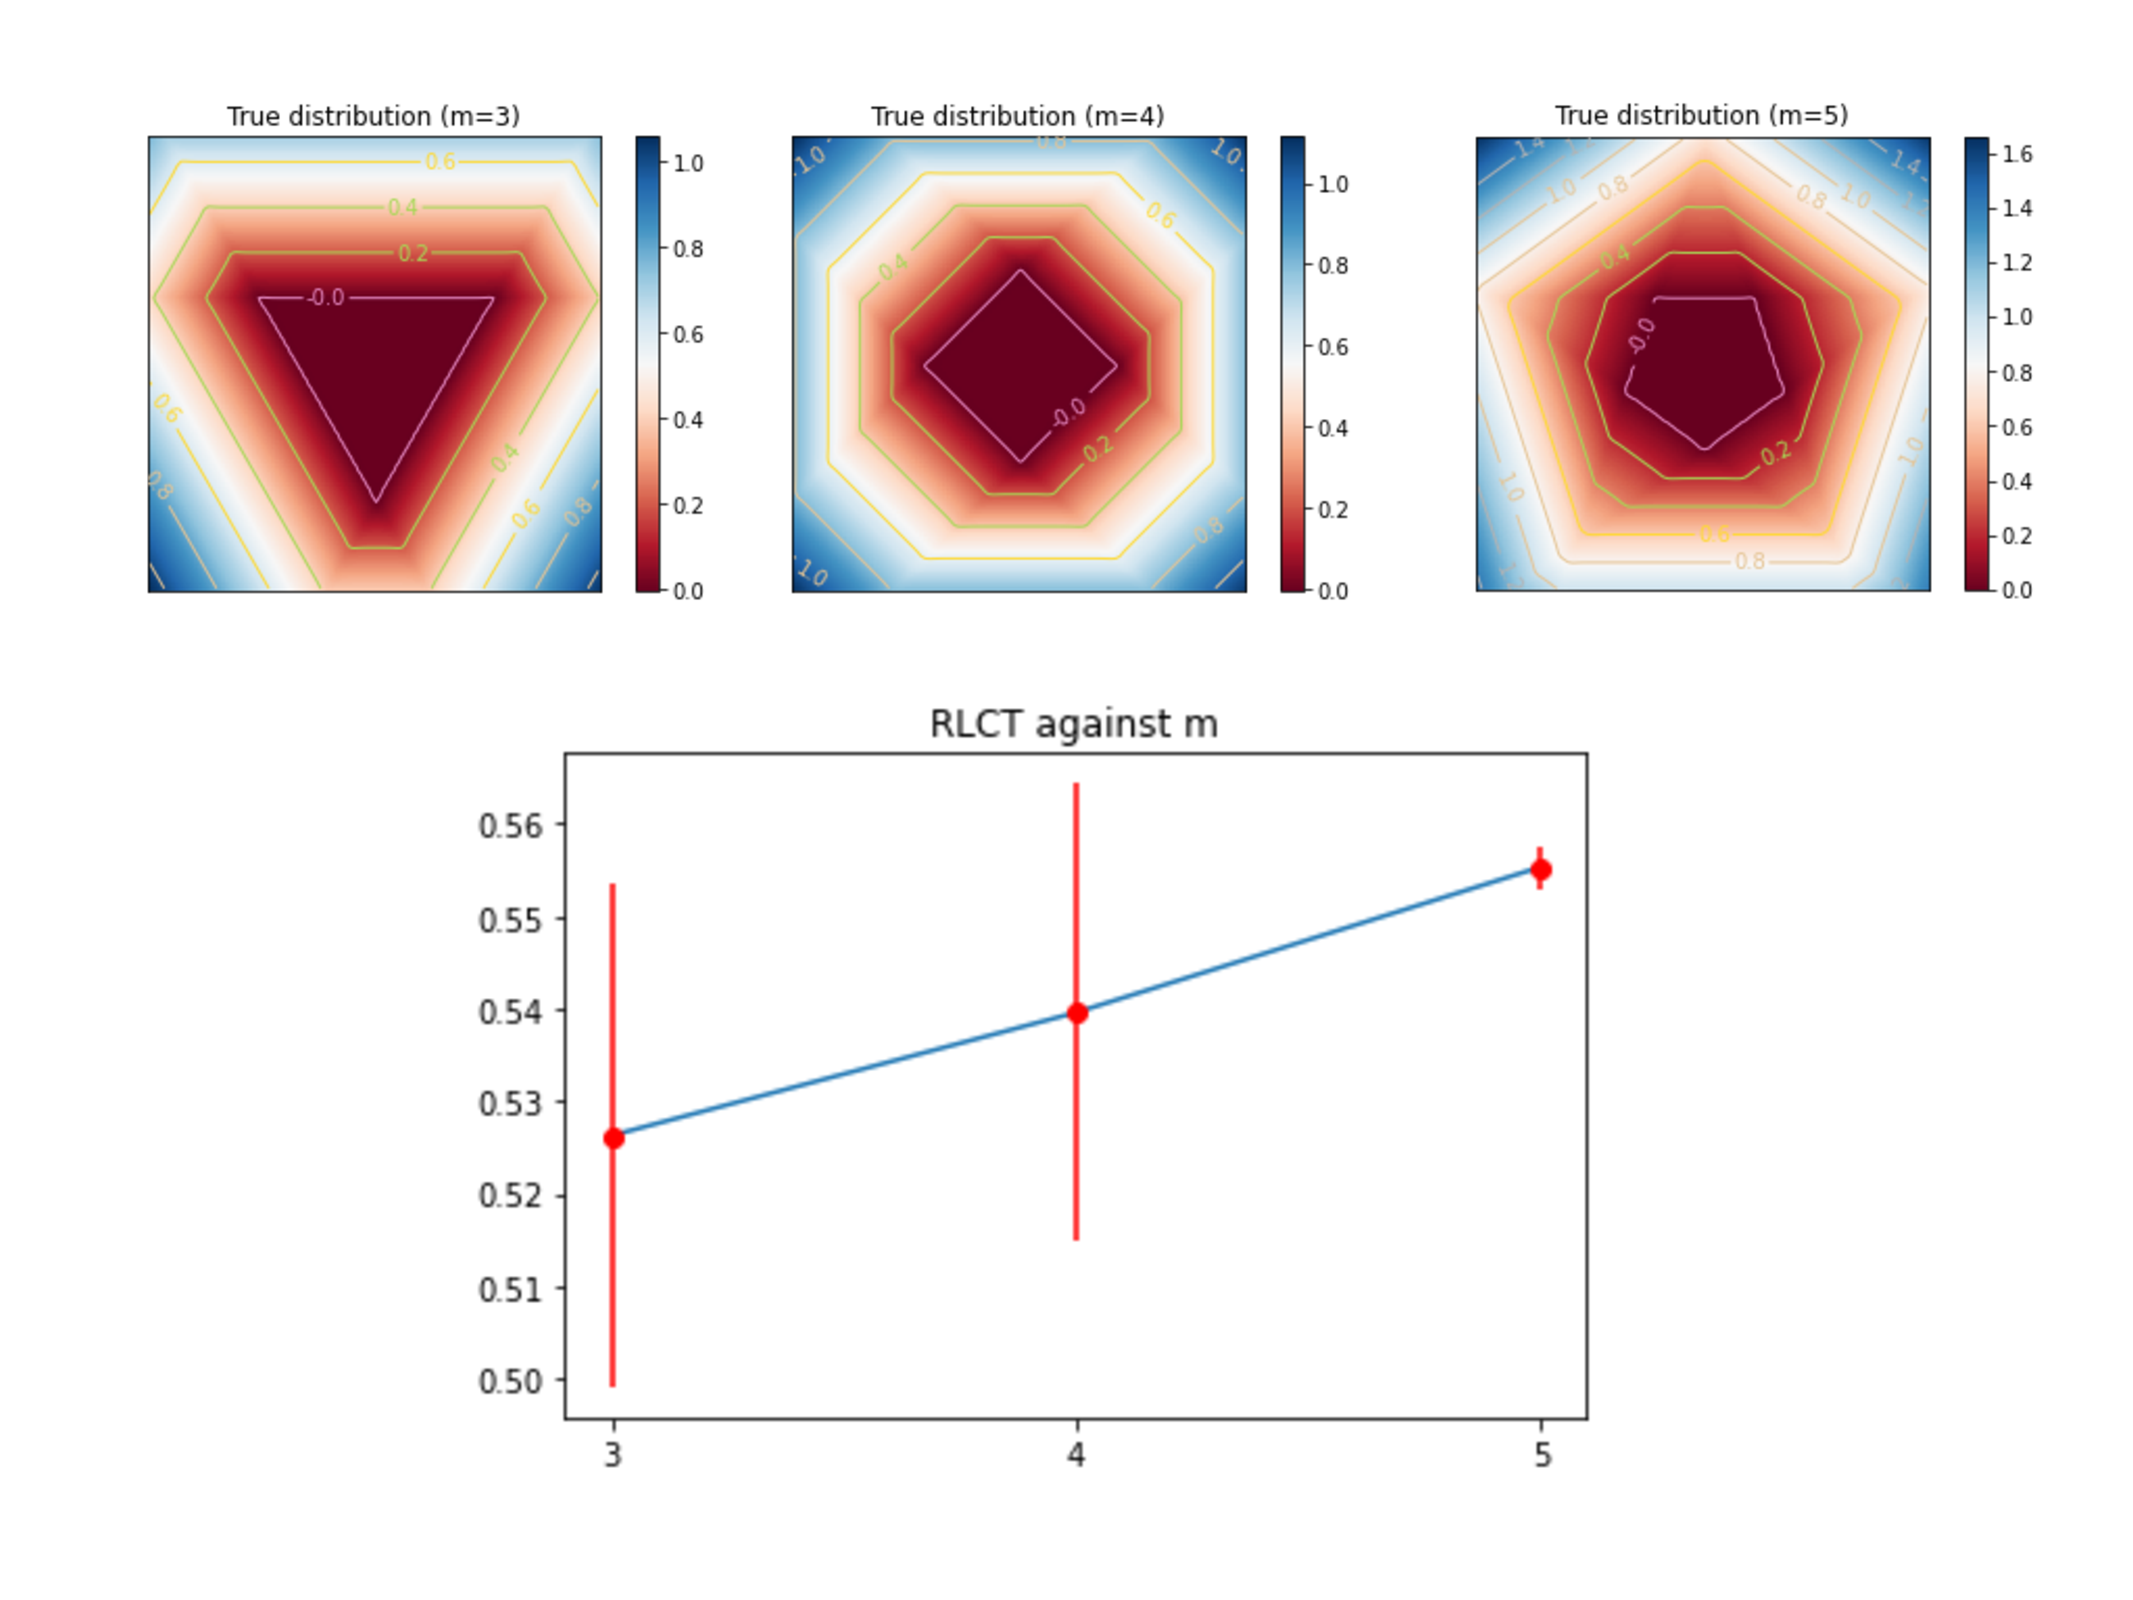
\includegraphics[scale=0.3]{RLCT_m.pdf}
\end{center}
\caption{Increasingly complicated true distributions $q(x,y)$ with a fixed model class, and the associated learning coefficients (TODO fix).}
\label{figure:simp_func_complex}
\end{figure}

The complexity of a singularity is inversely proportional to the RLCT so this predicts that as the true distribution becomes more ``complicated'', relative to the supposed model, the RLCT should increase. While in general it is not clear how to give an \emph{a priori} measure of function complexity other than the RLCT itself, we can construct simple examples in which such a measure is possible.

Consider a two-layer ReLU network
\begin{gather*}
f_\theta: \mathbb{R}^2 \longrightarrow \mathbb{R}\\
f_\theta(x) = c + \sum_{i=1}^H q_i \operatorname{ReLU}( \langle w_i, x \rangle + b_i )
\end{gather*}
where $\theta = (\{w_i\}_{i=1}^H, \{b_i\}_{i=1}^H, \{q_i\}_{i=1}^H, c) \in \mathbb{R}^{4H+1}$ and $w_i \in \mathbb{R}^2, b_i \in \mathbb{R}, q_i \in \mathbb{R}$ for $1 \le i \le H$. We let $W$ be some compact neighborhood of the origin in $\mathbb{R}^{3H+1}$ which contains all the networks that we are about to define. The statistical model $p(y|x,\theta)$ is defined by
\begin{equation}
p(y|x, \theta) = \frac{1}{\sqrt{2\pi}} \exp\Big( -\tfrac{1}{2} \| y - f_\theta(x) \|^2 \Big)
\end{equation}

Given an integer $3 \le m \le H$ we define a network $\kappa_m \in W$ and $q_m(y|x) := p(y|x, \kappa_m)$ as follows. Let $g \in SO(2)$ stand for rotation by $\frac{2\pi}{m}$, set $w_1 = g^{\tfrac{1}{2}} e_1$ where $e_i$ denote unit vectors. The components of $\kappa_m$ are defined as follows: $w_i = g^{i-1} w_1$ for $1 \le i \le m$ and $w_i = 0$ for $i > m$, $b_i = - \tfrac{1}{3}$ and $q_i = 1$ for $1 \le i \le m$ and $b_i = q_i = 0$ for $i > m$, and finally $c = 0$. Then the decision boundary for hidden node $i$ is the line $L_i = \{ x \in \mathbb{R}^2 \l \langle w_i, x - \tfrac{1}{3} w_i \rangle = 0 \}$ (the factor of $\tfrac{1}{3}$ ensures the relevant parts of the decision boundaries lie within $X = [0,1]^2$) and the distribution $q_m$ is $\mathbb{Z}/m\mathbb{Z}$-invariant. We let $q(x)$ be the uniform distribution on $X$ and define $q_m(x,y) = q_m(y|x) q(x)$. Let $\varphi$ be a normal distribution $\mathcal{N}(0,50^2)$ centered on $W$ and consider the RLCTs of the triples $(p, q_m, \varphi)$. 

Appendix \ref{appendix:RLCT_estimation} details the estimation procedure for the RLCT. The results are shown in Figure \ref{figure:simp_func_complex}.

We conducted the experiments with $H = 5$, $n = 1000$. The \emph{a posteriori} distribution was approximated by Hamiltonian Monte Carlo NUTS \cite{?} where the first 1000 steps were omitted and $20,000$ samples were collected. For each value of $m \in \{3,4,5\}$ three estimates of the RLCT were performed with the mean and standard deviation shown in Figure \ref{figure:simp_func_complex}. Each estimate was performed by linear regression on the pairs $\{ (1/\beta_i, \mathbb{E}^{\beta_i}_w[ nL_n(w) ] ) \}_{i=1}^5$ where the five inverse temperatures $\beta_i$ are centered on $1/\log(T)$ where $T = 20,000$. The theoretical justification for this estimation method is \citep[Theorem 4]{watanabe_widely_2013}. Note that in all cases the number of parameters in $W$ is $d = 21$ and the RLCTs are $< 1$, so not only are these models not regular, they are not even minimally singular (the dimension of the \emph{set} of true parameters, viewed as a submanifold, is $10$ when $m = 5$, so if this model were minimally singular the RLCT would have to be $11/2$).

The comments of \citep[\S 7.6]{watanabe_algebraic_2009} are based on the results of \citep[\S 7.2]{watanabe_algebraic_2009} which are summaries of \cite{??,??}. In \cite{??} the nonlinearity is the identity (reduced rank regression) and in \cite{??} the true distribution is always the zero function and the nonlinearity is $\operatorname{tanh}(x)$.

The RLCT estimates for the two-layer SiLU network (\ref{??}) provide evidence that this model is not minimally singular, when combined with the symmetric true distribution $q^{SiLU}_m(x,y)$. Starting from the weight vector of this true distribution, varying $c$ or any of the $b_i$ independently takes the model off the set of true parameters, so that the normal bundle has dimension $> H + 1$. Hence the RLCT in the minimally singular case would be bounded below by $3$ in the case $H = 5$, but our estimates for the RLCT are $< 0.6$.

We show in Appendix \ref{??} that when $m = H$ the set of true parameters $W_0 \subseteq W$ is a regular submanifold of dimension $m$. Hence if such a model is minimally singular its RLCT will be $\tfrac{1}{2}( (4m + 1) - m ) = \tfrac{1}{2}( 3m + 1 )$. In the case $m = 5$ we observe an RLCT more than an order of magnitude less than the value $8$ predicted by this formula.

\section{Future directions}
We claimed that the RLCT is \textit{the} correct way to account for model complexity in a deep neural network. We do not however claim that the RLCT can be easily estimated for a deep neural network. The intractability of RLCT estimation may not in reality be a significant deterrent. For instance, used in the context of model selection, the exact value of the RLCT is not as important as model selection consistency, i.e., if using the estimated RLCT leads to the same model being selected as if the true RLCT were being used. 

We have already illustrated that despite the fact that for very few singular models have theoretical RLCTs been catalogued, it is still possible to reap the insights offered by singular learning theory. In particular we showed that being Bayesian in the final layers, though a pale substitute for the full Bayes predictive distribution, nonetheless demonstrates humble improvements over point estimators. 
%\subsubsection*{Author Contributions}
%If you'd like to, you may include  a section for author contributions as is done
%in many journals. This is optional and at the discretion of the authors.
%
%\subsubsection*{Acknowledgments}
%Use unnumbered third level headings for the acknowledgments. All
%acknowledgments, including those to funding agencies, go at the end of the paper.


\bibliography{iclr2021_conference}
\bibliographystyle{iclr2021_conference}

\appendix
\section{Appendix}

\subsection{Estimating the RLCT using asymptotics}
\label{appendix:RLCT_estimation}

From derivations in \citep{watanabe_widely_2013}, we can glean several useful asymptotic characterisations of the RLCT. To set this up, we begin with some definitions. 
Let $L_n(w)$ be the negative log likelihood as in \eqref{eq:nll}. Define the data likelihood at inverse temperature $\beta >0$ to be $p^\beta(\mathcal D_n | w) = \Pi_{i=1}^n p(y_i |x_i, w)^\beta$, which can be written in terms of $L_n$ since
\begin{equation}
p^\beta(\mathcal D_n | w) = \exp(-\beta n L_n(w)).
\label{general_likelihood}
\end{equation}
The posterior distribution, at inverse temperature $\beta$, is defined as 
\begin{equation}
p^\beta(w|\mathcal D_n) = \frac{\Pi_{i=1}^n p(y_i|x_i,w)^\beta \varphi(w)}{\int_W \Pi_{i=1}^n p(y_i|x_i,w)^\beta \varphi(w)} = \frac{p^\beta(\mathcal D_n|w) \varphi(w)}{p^\beta(\mathcal D_n)}
\label{general_posterior}
\end{equation}
where $\varphi$ is the prior distribution on the network weights $w$ and
\begin{equation}
p^\beta(\mathcal D_n) = \int_W p^\beta(\mathcal D_n|w) \varphi(w) \,dw
\label{general_marginal_likelihood}
\end{equation}
is the marginal likelihood of the data at inverse temperature $\beta$. 

Finally, denote the expectation of a random variable $R(w)$ with respect to the tempered posterior $p^\beta(w|\mathcal D_n)$ as
\begin{equation}
{\E}_w^\beta [R(w)] = \int_W R(w) p^\beta(w|\mathcal D_n) \,dw
\label{general_expectation_posterior}
\end{equation}
% There are two senses to the estimation that is required of the real log canonical threshold. In the first sense, assuming the true distribution $q$ is known, we may be able to only approximate $\lambda(q)$. In the second sense, we msut grapple with the fact that $q$ is not known and the plug-in procedure $\lambda(\hat q)$ is not sound. Works addressing the former vein largely come from researchers well-versed in algebraic geometry \cite{lin_ideal-theoretic_2017,imai_estimating_2019} while statisticians tend to treat the second estimation aspect \cite{drton_bayesian_2017}.

Henceforth, when $\beta = 1$, we drop the superscript in the quantities \ref{general_likelihood}, \ref{general_posterior}, \ref{general_marginal_likelihood}, \ref{general_expectation_posterior}, e.g., $p(\mathcal D_n)$ rather than $p^1(\mathcal D_n)$. ???is this necessary???


Assuming the conditions of Theorem 4 in \cite{watanabe_widely_2013} hold, we have
\begin{equation}
    {\E}_w^\beta [nL_n(w)] = nL_n(w_0) + \frac{\lambda \log n}{\beta_0} + U_n \sqrt{\frac{\lambda \log n}{2 \beta_0}} + O_p(1)
    \label{eq:Theorem4_WBIC}
\end{equation}
where $\beta_0$ is a positive constant and $U_n$ is a sequence of random variables satisfying ${\E}_n U_n = 0$. %Assuming $q(y|x)$ is realisable (which we do), $U_n$ behaves nicely ???insert some of those nice properties???.
In Algorithm \ref{alg:thm4}, we describe an estimation procedure for the RLCT based on \eqref{eq:Theorem4_WBIC}.

To use any of these three asymptotic characterisations of $\lambda$, we need to compute integrals of the form $E_w^\beta [n L_n(w)]$. However, the $p^\beta(w|\mathcal D_n)$ is intractable for any $\beta>0$, rendering computation of $E_w^\beta$ challenging. For regular models, the Laplace approximation to ${\E}_w^\beta [R(w)]$ would be reasonable (as guaranteed for instance by the Berstein-von Mises theorem.) Recall the Laplace approximation in this case would replace ${\E}_w^\beta$ with an expectation with respect to a normal random variable with mean $w_0$, which is a mode of $L_n$, and covariance which is the Hessian $H_{ij} =\frac{\partial^2 L_n}{\partial w_i \partial w_j}$. But as we discussed earlier, for strictly singular models, the Laplace approximation does not hold. 

At present there does not exist a method of sampling from the Bayesian posterior for large neural networks which is sufficiently accurate to yield accurate RLCT estimates. Variants of MCMC are the gold standard for such estimations, but these techniques do not scale to large networks; consequently we restrict to small networks (TODO: death of local RLCT idea?)

\begin{algorithm}[tb]
	\caption{RLCT via Theorem 4}
	\label{alg:thm4}
	\begin{algorithmic}
		\STATE {\bfseries Input:} range of $\beta$'s, set of training sets $\mathcal T$ containing $M$ training sets of size $n$, approximate samples $\{w_1,\ldots,w_r\}$ from $p^\beta(w|\mathcal D_n)$ for each training set $\mathcal D_n$ and each $\beta$
		\FOR{training set $\mathcal D_n \in \mathcal T$}
    		\FOR{$\beta$ in range of $\beta_0/\log n$}
        		\STATE Approximate ${\E}_w^\beta [nL_n(w)]$ with $\frac{1}{r} \sum_{i=1}^r nL_n(w_r)$
    		\ENDFOR
    		\STATE Perform generalised least squares to fit $\lambda$ in \eqref{eq:Theorem4_WBIC}, call result $\hat \lambda^\beta(\mathcal D_n)$
		\ENDFOR
		\STATE {\bfseries Output:} $\frac{1}{M} \sum_{\mathcal D_n \in \mathcal T} \hat \lambda^\beta(\mathcal D_n)$
	\end{algorithmic}
\end{algorithm}

Very few theoretical RLCTs are known for strictly singular models. They are certainly not known for modern deep neural networks where the network weights number on the order of $n$. Furthermore singular learning theory, as it stands, cannot be directly applied to neural networks with the ReLU activation function. 

\subsection{Connection between RLCT and generalization} \label{appendix:generalization_theory}
For completeness, we sketch the asymptotic expansion of the average generalization error in singular models. The exposition is an amalgamation of various papers published by Sumio Watanabe, but mostly based on the textbook \cite{watanabe_algebraic_2009}. 

To understand the connection between the RLCT and $G(n)$, we first define the so-called \textbf{Bayes free energy} as 
\[
F(n) = -\log p(\mathcal D_n)
\]
whose expectation admits the following asymptotic expansion \cite{watanabe_algebraic_2009}
\[
{\E}_n F(n) =  {\E}_n n S_n + \lambda \log n + o(\log n)
\]
where $S_n = -\frac{1}{n} \sum_{i=1}^n \log q(y_i|x_i)$ is the entropy. This deceptively simple result is actually based on a set of sophisticated tools, in particular Hironaka's resolution theorem from algebraic geometry.

The expected Bayesian generalisation error can be connected to the Bayes free energy via the following relation:
\[
{\E}_n G(n) = \E F(n+1) - \E(F_n)
\]
Then we have the expected Bayes generalisation error is related to the RLCT as follows
\begin{equation}
{\E}_n G(n) = \lambda/n + o(1/n)
\label{eq:bayesgenerr}
\end{equation}
Since models with more complex singularites have smaller RLCTs, this would suggest that the more singular a model is, the better its generalization (assuming one uses the Bayesian predictive distribution for prediction). In this connection it is interesting to note that simpler true distributions lead to more singular models (Section \ref{section:simple_func}).

That the RLCT has such a simple relationship to the Bayesian generalisation error is remarkable. On the other hand, the practical implications of (\ref{eq:bayesgenerr}) are limited. This is because the Bayes predictive distribution in the case of a deep neural network is itself intractable. While we believe that approximations to the Bayesian predictive distribution, say via variational inference, might inherit a similar relationship between generalisation and the (variational) RLCT, serious theoretical developments will be required to rigorously establish this. The challenge comes from the fact that for approximate Bayesian predictors, the free energy and generalisation error have different learning coefficients $\lambda$. This was well documented in the case of a neural network with one hidden layer \citep{nakajima_variational_2007}. 

\subsection{Details for generalization error experiments}
\label{appendix:generalizaton}

\paragraph{Simulated data}
Input and target variables are both in $\mathbb R^3$. The distribution of $x$ is set to $q(x)=$ ???. We simulate the data under the realizability assumption, i.e. we draw $y$ given $x$ according to \eqref{eq:genexp_model} for some $w_0 \in W$, drawn randomly. ??? mention $x_test_std$.

\paragraph{Network architecture} In our experiments, $f = h \circ g$ where $g$ is a sequence of 
\[
\text{linear} \circ \text{ReLU} \circ \ldots \text{linear}
\]
and $h$ is either
\begin{equation}
    \text{linear} \circ \text{ReLU} \circ \text{linear} 
\end{equation}
or
\begin{equation}
    \text{linear}  \circ \text{linear}. 
\end{equation}
We fix the number of hidden units in $g$, the feedforward ReLU block, to 5 and the number of hidden units in $h$, the last two years, to 3. We varied the number of layers in $g$ between $1$ and $5$.

\paragraph{MAP training}
The MAP estimator is found via stochastic gradient descent on the MSE loss with minibatch set to ???. Training was set to 5000 epochs with no early stopping. 

\paragraph{Calculating the generalization error}
We calculate the average generalization error using a held-out-test set $T_{n'} = \{(x_i',y_i')\}_{i=1}^{n'}$ as
\begin{equation}
\frac{1}{n'} \sum_{i=1}^{n'} \log q(y_i'|x_i') - {\E}_n \frac{1}{n'} \sum_{i=1}^{n'} \log \hat q_n(y_i'|x_i')
\label{eq:computed_avgGn}
\end{equation}
Assume the held-out test set is large enough so that the difference between ${\E}_n G(n)$ and \eqref{eq:computed_avgGn} is negligible. We will refer to them interchangeably as the average generalization error. 

\paragraph{Laplace in the last layer(s)}
Describe Laplace in last layer and reduced regression layers.


\paragraph{MCMC in the last layer(s)}
 Let $\tilde x_i = g_{v_{map}}(x_i)$. Define a new transformed dataset $\tilde{\mathcal D_n} = \{(\tilde x_i, y_i) \}_{i=1}^n$. We perform MCMC to sample the posterior over $w$:
$$
p(w | \tilde{\mathcal D_n}) \propto p(\tilde{\mathcal D_n} | w) \varphi(w) = \Pi_{i=1}^n \exp\{-|| y_i - h_w \circ g_{v_{map}}(x_i) ||^2/2\} \varphi(w)
$$

Define the following approximation to the Bayesian predictive distribution
$$
\tilde p(y|x, \mathcal D_n) = \int p(y|x,(v_{map},w)) p(w|\tilde{\mathcal D_n}) \,dw
$$
We use HMC (NUTS variant) \citep{hoffman2014no} to draw $w_1,\ldots,w_R$ from $\tilde{\mathcal D_n}$. Then we approximate $\textbackslash\{\}tilde p(y|x, \textbackslash\{\}mathcal D\_n)$ with
\[
\frac{1}{R} \sum_{r=1}^R p(y|x,(v_{map},w_r))
\]
where $R$ is a large number, set to ???1000??? in our experiments.

%We have to be careful when we speak of the generalization error of the approximate predictive distribution above. For a proper comparison to ${\E}_n G_{map}(n)$ or ${\E}_n G_{mle}(n)$, we have to look at 
%\begin{equation}
%{\E}_n G_{mcmcrr}(n) =  KL (q(y|x) || p_{mcmcrr}(y|x, \mathcal D_n) )
%\label{G_LLB}
%\end{equation}
%where ${\E}_n$ averages out the randomness of both $D_n$ and  $v_{map}$. 
%
%An alternative is to condition on $v_{map}$, using $g_{v_{map}}$ as a feature extractor in a preprocessing step. Then, assuming realizability $q(y|x) = p(y|x,(v_0,w_0))$ we may examine the generalizaton error
%\begin{equation}
%E_{\mathcal D_n | v_{map}} KL( p(y|x,(v_{map},w_0)) || p_{mcmcrr}(y|x, \mathcal D_n) )
%\label{G_LLB_vfixed}
%\end{equation}
%The average generalization error in \eqref{G_LLB_vfixed} is distinctly different from the one in \eqref{G_LLB}. The nice thing about \eqref{G_LLB_vfixed} is that we know its asymptotic expansion is $\lambda/n$ where $\lambda$ corresponds to the triplet $( p(y|x,(v_{map},w_0)), p(y| x, (v_{map},w)), \varphi(w))$. For certain functions $h_w$ where the true $\lambda$ is known, we can verify this in the experiments. (Not implemented yet).


\end{document}
